\chapter{Industrialisation du produit}
\label{Industrialisation du produit}
\thispagestyle{fancy}
Une fois le processus fonctionnel de notre système défini, on l'industrialise. Cela signifie que l'on crée un ensemble d'outils qui permettent de l'utiliser de la manière la plus simple possible et ce en répondant au mieux à la problématique initiale. \\
On soumet deux types d'outils: l'API, qui permet d'utiliser le système d'automatisation et les outils graphiques, qui accompagnent l'usage de l'API et offrent à l'utilisateur un moyen d'interagir avec le programme.  

\section{API}
\label{Industrialisation du produit: API}
L'API que l'on propose est composée de 3 modules :
\begin{description}
	\item [data base] Permet de gérer le stockage et la lecture des données nécessaires à l'exécution des algorithmes d'apprentissage. Deux types de fichiers y sont sauvegardés : les fichiers logs, qui fournissent l'ensemble des exemples permettant d'entraîner le SVM et les fichiers générés par l'algorithme lors de son apprentissage.
	\item [data set] Permet de prétraiter les exemples utilisés pour l'apprentissage.
	\item [machine learning] Permet de créer un algorithme d'apprentissage, de l'entraîner et de l'utiliser pour investiguer la \emph{root cause} pour laquelle il a été créé.
\end{description}

La librairie utilise le langage de programmation Python \cite{Python}. \\

\subsection{Prétraitement des données}
\label{Industrialisation du produit: API: Pré-traitement et traitement des données}
Le module "Data set" de l'API permet de prétraiter les exemples et de les structurer pour entraîner le SVM. 
Le prétraitement est composé de 5 étapes.
\begin{description}
	\item [Lecture] Lecture des données contenues dans le fichier log. 
	\item [Échantillonnage] Les fichiers logs générés par MEIGUI lors du déroulement du Filtering Test n'ont pas forcement tous la même période d'échantillonnage. Cela signifie que les exemples que l'on souhaite utiliser pour l'entraînement ne font pas tous la même taille. Or, les spécificités des fonctions de la librairie Scikit-learn utilisées pour l'entraînement nécessite que celles-ci aient le même nombre d'échantillons. Pour cette raison, on échantillonne les données extraites des fichiers logs ou le même nombre d'échantillons. Si le nombre d'échantillons contenus dans le fichier log est inférieur au nombre d'échantillons fixé par l'échantillonnage, on effectue un sur-échantillonnage, quand celui-ci n'altère pas les données. 
	\item [Selection des motifs] Au regard de l'architecture fonctionnelle que l'on a définie en partie \ref{Automatisation du processus d'investigation: Achitecture High Level du système proposé}, on doit extraire les motifs caractéristiques d'une root cause dans chaque exemple utilisé. Pour cela, une sélection manuelle du motif est réalisée en amont via une interface graphique (cf. \ref{Industrialisation du produit: Outils graphiques: Pattern selection}). A partir des informations retournées par l'IHM (Interface Homme Machine), on est en mesure de sélectionner les portions des exemples qui correspondent aux motifs. On rappelle que l'on sauvegarde également des morceaux de la courbe ne contenant pas de motif caractéristique d'une \emph{root cause}. Cette étape permet également de labelliser les exemples, i.e. indiquer si le motif sélectionné correspond à un motif caractéristique de la \emph{root cause}.
	\item [Déroulement des données] On déroule ensuite les données pour réaliser de la reconnaissance de motifs avec plusieurs features, i.e. que l'on place chacune des colonnes de notre matrice d'exemples les en dessous des autres. On obtient en sortie un vecteur. 
	\item [Tri des données] Enfin, pour mesurer les performances de notre algorithme (cf. partie \ref{Automatisation du processus d'investigation: Performances de la solution}), on sépare notre base de données d'exemples en deux groupes: le \emph{training set} et le \emph{test set}. Le premier sera utilisé pour entraîner notre algorithme, le deuxième pour le tester. 
\end{description}

\subsubsection{Sélection des motifs}
\label{Industrialisation du produit: API: Sélection des motifs}
Comme étudié en partie \ref{Automatisation du processus d'investigation: Reconnaissance de motifs}, la reconnaissance de motifs passe par la sélection des motifs caractéristiques de la root cause que l'on souhaite détecter, dans chaque exemple de notre base de données. Elle s'accompagne également de  la sélection de sections de la courbe ne présentant pas ce motif afin de pouvoir réaliser l'apprentissage de l'algorithme de manière optimale ( cf. partie \ref{Automatisation du processus d'investigation: Difficultés notoires rencontrées}).\\
 Chaque motif sélectionné doit avoir la même taille i.e. le même nombre d'échantillons pour pouvoir réaliser l'entrainement. Cette taille dépend de la largeur globale du motif caractéristique et est déterminée par l'utilisateur lors de l'utilisation de l'interface graphique présentée partie \ref{Industrialisation du produit: Outils graphiques: Pattern selection}.   

\subsubsection{Format des données de sortie}
\label{Industrialisation du produit: API: Format des données de sortie}
On présente dans le tableau \ref {tab: Structure de la base de données d'exemples après prétraitement} la structure des données en sortie du prétraitement des données. On a deux vecteurs : l'un contenant les exemples de motifs, l'autre contenant le label associé à chaque motif. Le label 1 signifie que le motif correspond à un motif caractéristique de la \emph{root cause} ; 0 signifie que le motif ne correspond pas à un motif caractéristique de la \emph{root cause}. 
\begin{equation}
\begin{blockarray}{cc}
exemples & labels \\
\begin{block}{[c][c]}
exemple_1 &  1 \\
exemple_2 & 0 \\
exemple_3 & 0 \\
exemple_4 & 1 \\
... & ... \\
exemple_m & 0 \\
\end{block}
\end{blockarray}
\label {tab: Structure de la base de données d'exemples après prétraitement}
\end{equation}
On retrouve cette structure pour chaque \emph{set} (i.e. \emph{training set} et \emph{test set}). \\
Chaque exemple correspond à une liste qui contient l'ensemble des échantillons contenus dans un motif.

\subsection{Module Marchine Learning}
\label{Industrialisation du produit:  API: Le module Machine Learning}
Le module Machine Learning s'appuie sur l'utilisation de scikit-learn \cite{ScikitLearn}. Il s'agit d'une bibliothèque Open Source développée par l'INRIA (Institut National de Recherche en Informatique et en Automatique \cite{INRIA}). Elle propose de nombreux outils qui permettent de réaliser de la classification (régression logistique, SVM), de la régression (SVR, régression linéaire) et du clustering (i.e. apprentissage non supervisé). On l'utilise dans le cadre de notre projet pour réaliser de classification (i.e. apprentissage supervisé) en utilisant l'algorithme d'apprentissage automatique SVM. Elle est également utilisée afin de construire le \emph{training set} et le \emph{test set} et déterminer les performances de l'algorithme.




\section{Outils graphiques}
\label{Industrialisation du produit: Outils graphiques}
On présente ici les différents outils graphiques qui permettent de réaliser la construction d'une nouvelle couche root cause (i.e. un nouvel algorithme pour détecter une \emph{root cause}), d'investiguer une \emph{error name} et d'obtenir des informations sur les performances de l'algorithme. 

\subsection{Pattern selector}
\label{Industrialisation du produit: Outils graphiques: Pattern selection}
Cet outil graphique permet de sélectionner les motifs contenus dans chaque exemple du \emph{training set} lors la phase de prétraitement  et de labellisation des exemples. \\
Il est formé de trois parties:
\begin{itemize}
	\item La première partie (encadré vert de la figure \ref{fig:Interface graphique du pattern selector}) nous fournit des informations sur l'état actuel du prétraitement des données : la taille du motif sélectionné, le nom de l'exemple étudié et le nombre d'exemples restant à traiter. 
	\item La seconde partie (encadré rouge de la figure  \ref{fig:Interface graphique du pattern selector}) affiche les features de l'exemple actuellement étudié. Dans le cas de la figure  \ref{fig:Interface graphique du pattern selector}, on réalise par exemple l'entraînement de l'algorithme pour que celui-ci puisse reconnaître le motif caractéristique de la root cause "frottement des freins de la hanche". La région en rouge permet de sélectionner le motif qui nous intéresse.
	\item La dernière partie (encadré bleu de la figure  \ref{fig:Interface graphique du pattern selector}) est une succession de boutons qui permettent à l'utilisateur d'interagir avec les différents exemples. De gauche à droite :   
	\begin{itemize}
		\item Le  bouton "Previous" permet de revenir à l'exemple précédent.
		\item Le bouton "Found" permet d'indiquer au système que le motif est présent sur l'exemple étudié, et qu'il a bien été sélectionné grâce à la région de sélection. Cela revient à labelliser l'exemple (Y = 1, cf. partie \ref{Industrialisation du produit: API: Format des données de sortie}). Le prochain exemple à étudier s'affiche.
		\item Le bouton "Not Found" permet d'indiquer au système que le motif n'est pas présent sur l'exemple étudié. Cela revient à labelliser l'exemple (Y = 0, cf. partie \ref{Industrialisation du produit: API: Format des données de sortie}). Le prochain exemple à étudier s'affiche.
		\item Le bouton en forme d'œil ouvert permet d'activer le mode étendu (cf. figure \ref{fig:Interface graphique du pattern selector en mode étendu}).
	\end{itemize} 
\end{itemize} 

\begin{figure}[H]
	\centering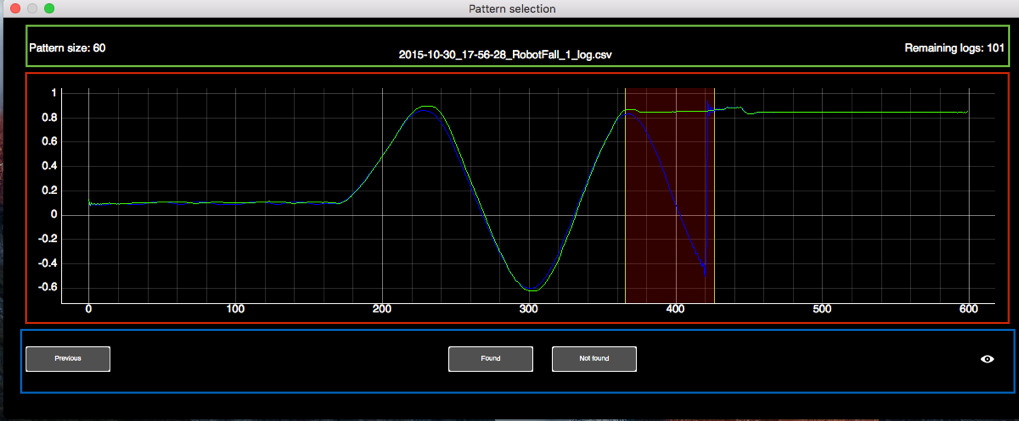
\includegraphics[height=6.4cm]{images/pattern_selector.png}
	\caption[Interface graphique du pattern selector]{Interface graphique du pattern selector.}
	\label{fig:Interface graphique du pattern selector}
\end{figure}

\subsubsection{Région de sélection}
\label{Industrialisation du produit: Outils graphiques: Pattern selection: La région de sélection}
La région de sélection permet de sélectionner le motif caractéristique d'une \emph{root cause} dans chaque exemple où celui-ci se présente. \\
 Il est possible d'augmenter la taille de celui-ci si le besoin est présent. Par exemple, imaginons que l'on sélectionne sur le premier exemple un motif, dont la taille est de 60 échantillons. On clique sur le bouton "Found" et un nouvel exemple s'affiche. Celui-ci contient également le motif caractéristique de la \emph{root cause} que l'on apprend. Cependant, ce dernier est plus large de 10 échantillons. Il est alors possible d'étendre la région de sélection pour pouvoir sélectionner l'ensemble de ce nouveau motif. Cependant, l'ensemble des exemples devant avoir la même taille (même nombre d'échantillons), on modifie la taille des motifs précédemment sélectionnés. Dans le cas de notre exemple, on augmente la taille du motif précédent de 5 échantillons de chaque côté. \\
Il n'est pas possible de réduire la taille d'un motif, pour ne pas perdre des données sur les exemples précédemment sélectionnés. 

\subsubsection{Mode étendu}
\label{Industrialisation du produit: Outils graphiques: Pattern selection: Mode étendu}
Il existe certains cas où les valeurs de deux features étudiées sont trop éloignées l'une de l'autre pour pouvoir être visualisées de manière correct. Pour cela, on peut basculer l'IHM en mode étendu, ce qui permet d'afficher chacune des features dans un graphique séparé. La région de sélection est commune aux différents graphe, i.e. sa taille et sa position sont contrôlées via le graphique principal et se répercutent sur les graphitiques du mode étendu (cf. figure \ref{fig:Interface graphique du pattern selector en mode étendu})

\begin{figure}[H]
	\centering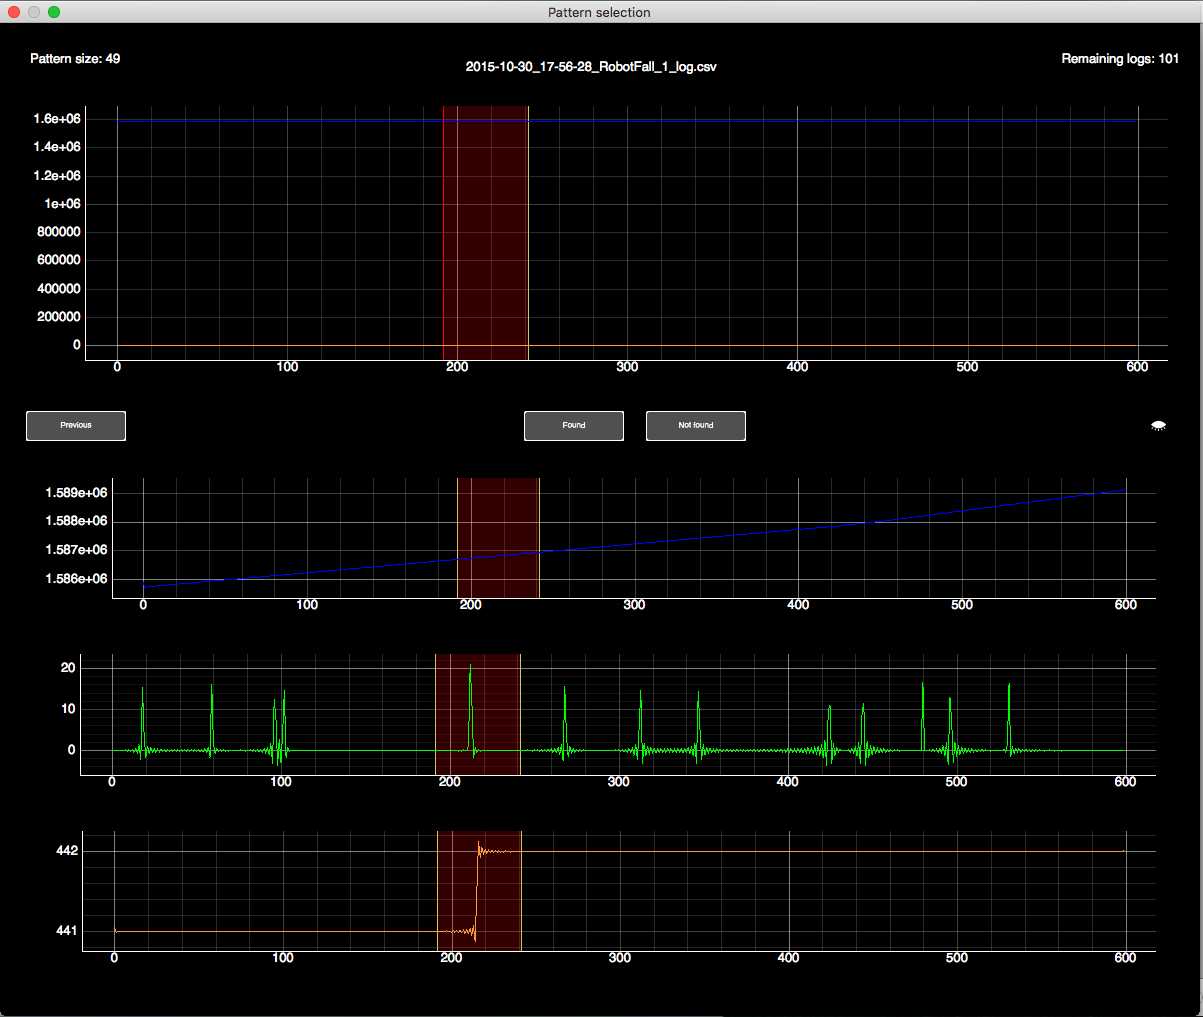
\includegraphics[height=9cm]{images/pattern_selector_ext.png}
	\caption[Interface graphique du pattern selector en mode étendu]{Interface graphique du pattern selector en mode étendu. On observe sur ce graphique les trois features BackPlateformAck, BackPlateformNack et BackPlateformError du premier exemple. On remarque que l'affichage sur le graphique principal n'est pas clair. Le mode étendu permet d'afficher chacune des features. La région de sélection est commune aux trois graphiques (même position, même taille).}
	\label{fig:Interface graphique du pattern selector en mode étendu}
\end{figure}

\subsection{Probability Visualization}
\label{Industrialisation du produit: Outils graphiques: Probability Visualization}
Cette interface graphique permet de visualiser l'exemple que l'on investigue et la probabilité que le motif soit présent dans l'image. Elle est composée de deux parties. 
\begin{itemize}
	\item La première partie (encadré vert sur la figure \ref{fig:Interface graphique du probability visualizator}) affiche les features de l'exemple que l'on investigue. Par exemple, dans le cas présent, on recherche la \emph{root cause} liée à l'\emph{error name} "chute du robot". Le système détecte que la \emph{root cause} est "le frottement des freins de la hanche". Il nous affiche donc les courbes du senseur et de l'actuateur de la hanche, sur lesquelles on observe le motif caractéristique de la \emph{root cause}. 
	\item La deuxième partie (encadré rouge sur la figure \ref{fig:Interface graphique du probability visualizator}) affiche la courbe de progression de la probabilité, au cours du balayage des features de l'exemple (cf. partie \ref{Automatisation du processus d'investigation: Reconnaissance de motifs: Concept}). La ligne horizontale sur le graphique représente le seuil à partir duquel on considère que la \emph{root cause} est bien la cause ayant entraîné l'apparition de l'erreur.
\end{itemize}

\begin{figure}[h]
	\centering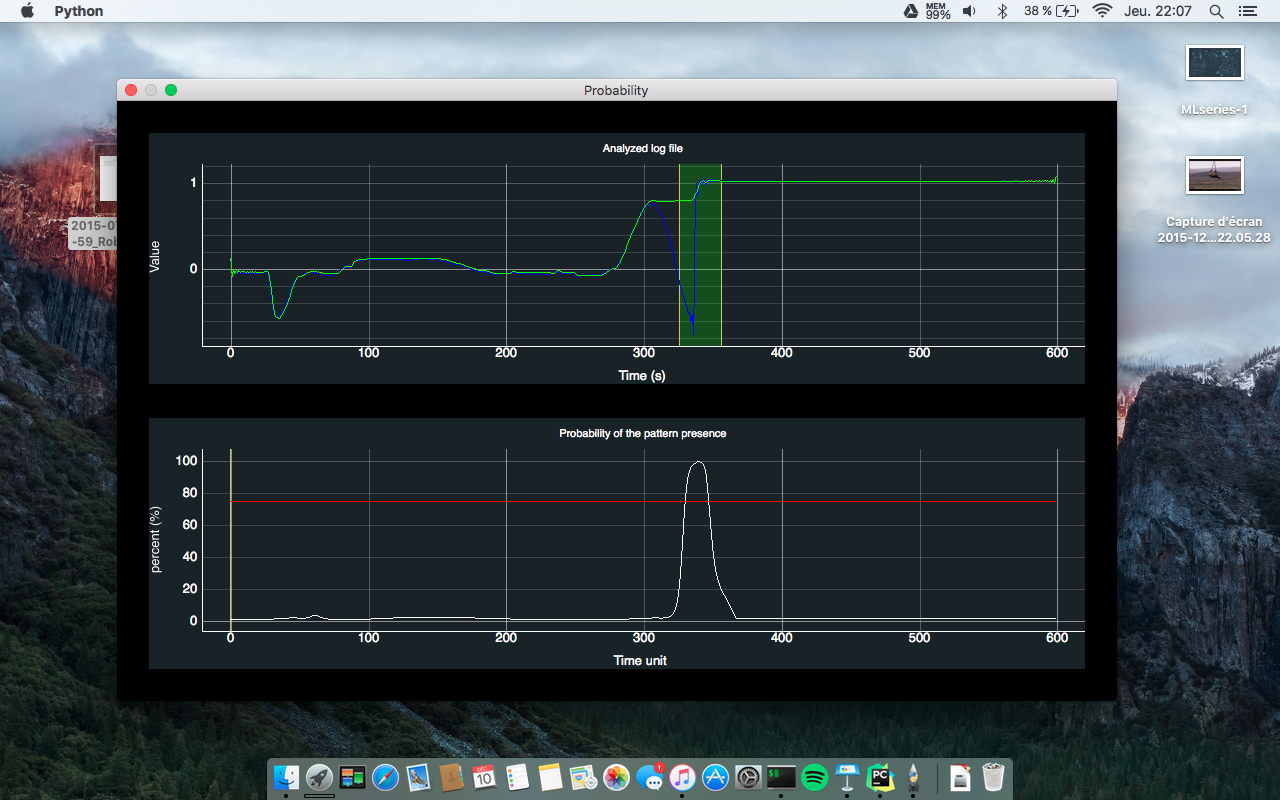
\includegraphics[height=7cm]{images/proba_visu.png}
	\caption[Interface graphique du probability visualizator]{Interface graphique du probability visualizator.}
	\label{fig:Interface graphique du probability visualizator}
\end{figure}

\subsection{Control panel}
\label{Industrialisation du produit: Outils graphiques: Control panel}
Le control panel permet d'obtenir un certain nombre d'informations quant à la qualité de la base de données d'exemple utilisée pour créer une nouvelle couche \emph{root cause}, ainsi que sur les performances de l'algorithme d'apprentissage automatique. La plupart de ces informations sont déterminées grâce aux outils soumis en partie \ref{Automatisation du processus d'investigation: Performances de la solution}. L'IHM est composé de trois parties.
\begin{description}
	\item [Data set features] (encadré vert sur la figure \ref{fig:Interface graphique du control pattern}) fournit un ensemble d'informations sur la base de données d'exemples utilisée pour l'entraînement de l'algorithme d'apprentissage automatique. 
	\item [Training panel features ](encadré rouge sur la figure \ref{fig:Interface graphique du control pattern})  livre des informations sur l'algorithme d'apprentissage automatique de la couche root cause analysée (e.g. valeur des paramètres, matrice de confusion, précision, etc). Ces données sont pour la plupart relatives aux explications fournies en partie \ref{Automatisation du processus d'investigation: Performances de la solution}.
	\item [Training panel ](encadré bleu sur la figure \ref{fig:Interface graphique du control pattern}) permet d'analyser les courbes d'apprentissage (c.f. partie \ref{Industrialisation du produit: Performances de la solution:Courbes d'apprentissage}) et les courbes de validation (c.f. partie \ref{Industrialisation du produit: Performances de la solution:Optimisation des paramètres du SVM})
\end{description}

\begin{figure}[H]
	\centering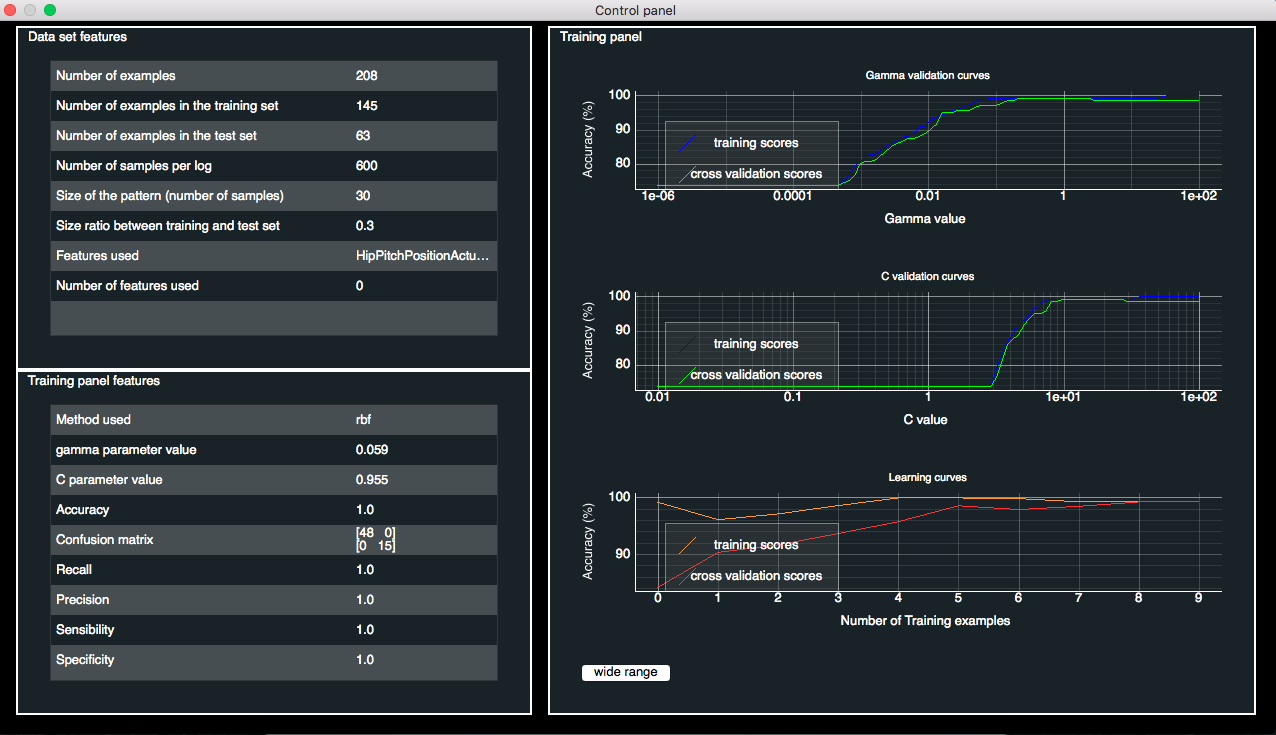
\includegraphics[height=7cm]{images/control_panel.png}
	\caption[Interface graphique du control pattern]{Interface graphique du control pattern.}
	\label{fig:Interface graphique du control pattern}
\end{figure}

\section{Utilisation suggérée des outils}
\label{Industrialisation du produit: Utilisation suggérée des outils}
On propose dans cette partie un exemple d'utilisation de l'API et des interfaces graphiques. Cette solution a été mise en place dans le cadre du stage afin de proposer un script qui permet d'ores et déjà de gérer la base de données, de créer de nouvelles couches \emph{root cause} et d'investiguer des fichiers logs. On s'appuie sur l'utilisation de la libraire python \emph{npyscreen} \cite{Npyscreen} qui permet de réaliser des interfaces utilisateurs simples, directement dans le terminal.
\newline

On s'intéressera ici au problème de frottement des freins de la hanche, qui entraîne la chute du robot durant le Filtering Test. Sa résolution passe donc par trois étapes: 
\begin{enumerate}
	\item Créer une nouvelle couche \emph{error name} : la couche "chute du robot". 
	\item Créer un nouvelle couche \emph{root cause} liée à la couche \emph{error name} "chute du robot" : la couche "frottement des freins de la hanche". Cela signifie que l'on va entraîner un nouvel algorithme à détecter le motif caractéristique de cette \emph{root cause}. 
	\item vérifier les performances de la nouvelle couche \emph{root cause} créée via le Control Panel.
	\item Investiguer un fichier log. 
\end{enumerate}

\subsection{Menu principal}
\label{Industrialisation du produit: Utilisation suggérée des outils: Menu principal}
Le menu principal (cf. figure \ref{fig:Menu principal}) permet d'ouvrir 5 sous-menus qui permettent respectivement de :
\begin{itemize}
	\item Créer une nouvelle couche \emph{error name} et l'ajouter à la base de données.
	\item Créer une nouvelle couche \emph{root cause}, la lier à une couche \emph{error name} et l'ajouter à la base de données.
	\item Investiguer un fichier log
	\item Mettre à jour une \emph{root cause}
	\item Ouvrir le control panel
\end{itemize}

\begin{figure}[H]
	\centering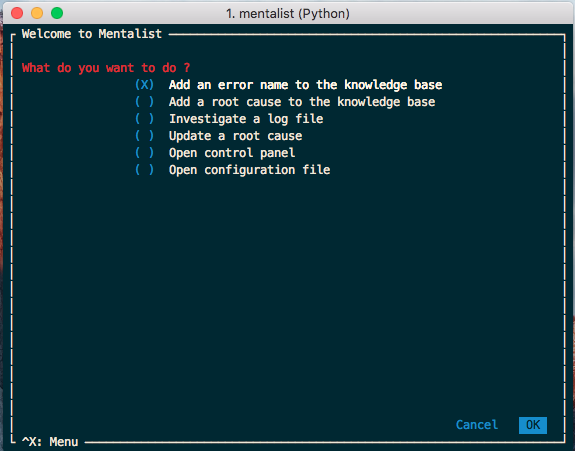
\includegraphics[height=7cm]{images/main_menu.png}
	\caption[Menu principal]{Menu principal.}
	\label{fig:Menu principal}
\end{figure} 

\subsection{Nouvelle error name}
\label{Industrialisation du produit: Utilisation suggérée des outils: Nouvelle error name}
Le menu "Add an error name to the knowledge base" (cf. figure \ref{fig:Menu principal}) permet d'ajouter une couche \emph{error name} dans la base de données. \\
Il suffit pour cela d'indiquer le nom de la couche \emph{error name} que l'on souhaite créer: dans notre cas, on l'appellera \textbf{fall down}. Celle-ci ne contient alors aucune \emph{root cause}.

\subsection{Nouvelle root cause}
\label{Industrialisation du produit: Utilisation suggérée des outils: Nouvelle root cause}
Le menu "Add a root cause to the knowledge base" (cf. figure \ref{fig:Menu principal}) permet de créer une nouvelle \emph{root cause} (i.e. entraîner un nouvel algorithme d'apprentissage à reconnaître une \emph{root cause}), à la lier à une couche \emph{error name}, et à l'ajouter à la base de données. \\
Pour cela, on suit le processus suivant (cf. figure \ref{fig: Nouvelle root cause}) : 
\begin{enumerate}
	\item On sélectionne l'\emph{error name} à laquelle on souhaite lier cette nouvelle \emph{root cause}. On indique ensuite son nom. Dans le cas de la \emph{root cause} "frottement des freins de la hanche", on la lie à l'\emph{error name} "fall down" et on l'appelle "frottement des freins de la hanche". 
	\item On sélectionne la/les feature(s) liée(s) à la \emph{root cause}. Dans le cas de la \emph{root cause} du "frottement des freins de la hanche", on sélectionne les clés HipPitchPositionSensorValue, HipPitchPositionActuatorValue, respectivement les valeurs du senseur et de l'actuateur de la hanche. 
	\item On utilise le Pattern Selector (cf. partie \ref{Industrialisation du produit: Outils graphiques: Pattern selection}) pour sélectionner les motifs caractéristiques de la \emph{root cause} que l'on étudie. Dans notre cas, il s'agit du moment où le senseur ne suit plus l'actuateur. On répète cette manipulation pour chaque exemple de la base de données.
\end{enumerate}

\begin{figure}[H]
	\centering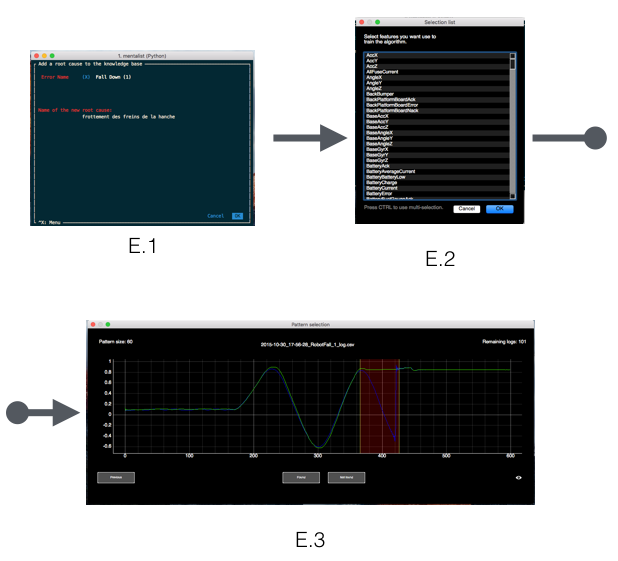
\includegraphics[width=10cm]{images/add_root_menu.png}
	\caption[Nouvelle root cause]{Nouvelle root cause.}
	\label{fig: Nouvelle root cause}
\end{figure} 


\subsection{Investiguer un fichier log}
\label{Industrialisation du produit: Utilisation suggérée des outils: Investiguer}
Le menu "Investigate a log file" (cf. figure \ref{fig:Menu principal}) permet de réaliser une investigation sur un fichier log, i.e. trouver la root cause ayant entraîné l'apparition de l'error name durant le Filtering Test. Pour cela, on suit le processus suivant (cf. figure \ref{fig: Investigation d'un fichier log}) : 
\begin{enumerate}
	\item On commence par indiquer au script le chemin vers le fichier log. On sélectionne ensuite l'error name que l'on souhaite investiguer, dans la liste des errors name connues (i.e. présentes dans la base de données).
	\item Le programme nous affiche le Probability Visualizator (cf. partie \ref{Industrialisation du produit: Outils graphiques: Probability Visualization})
	\item Une fois le Probability Visualizator fermé, le script nous indique la root cause trouvée dans le fichier log. 
\end{enumerate}

\begin{figure}[H]
	\centering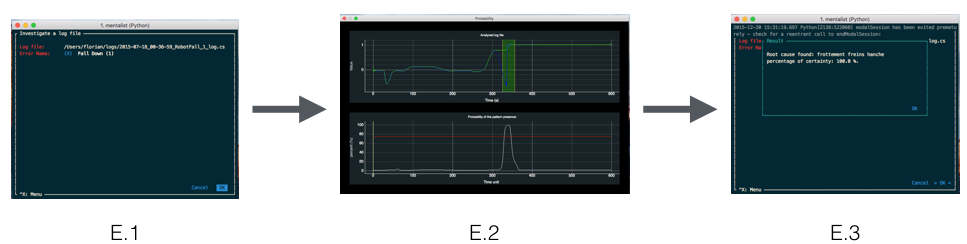
\includegraphics[width=10cm]{images/invest_menu.png}
	\caption[Investigation d'un fichier log]{Investigation d'un fichier log.}
	\label{fig: Investigation d'un fichier log}
\end{figure} 

\subsection{Analyse des performances d'une  root cause}
\label{Industrialisation du produit: Utilisation suggérée des outils: Analyse des performances d'une  root cause}
Le menu "Open control panel" (cf. figure \ref{fig:Menu principal}) permet de sélectionner une root cause liée à une error name et d'en afficher le control panel pour obtenir des informations sur la qualité des exemples utilisés pour l'apprentissage automatique et sur les performances. Pour cela, on suit le processus suivant (c.f. figure \ref{fig: Analyse des performances d'une couche root cause}) : 
\begin{enumerate}
	\item On sélectionne dans l'arborescence des \emph{errors name} et des\emph{ root causes}, la \emph{root cause} que l'on souhaite étudier.
	\item Le Control Panel s'affiche (cf. partie \ref{Industrialisation du produit: Outils graphiques: Control panel})
\end{enumerate}

\begin{figure}[H]
	\centering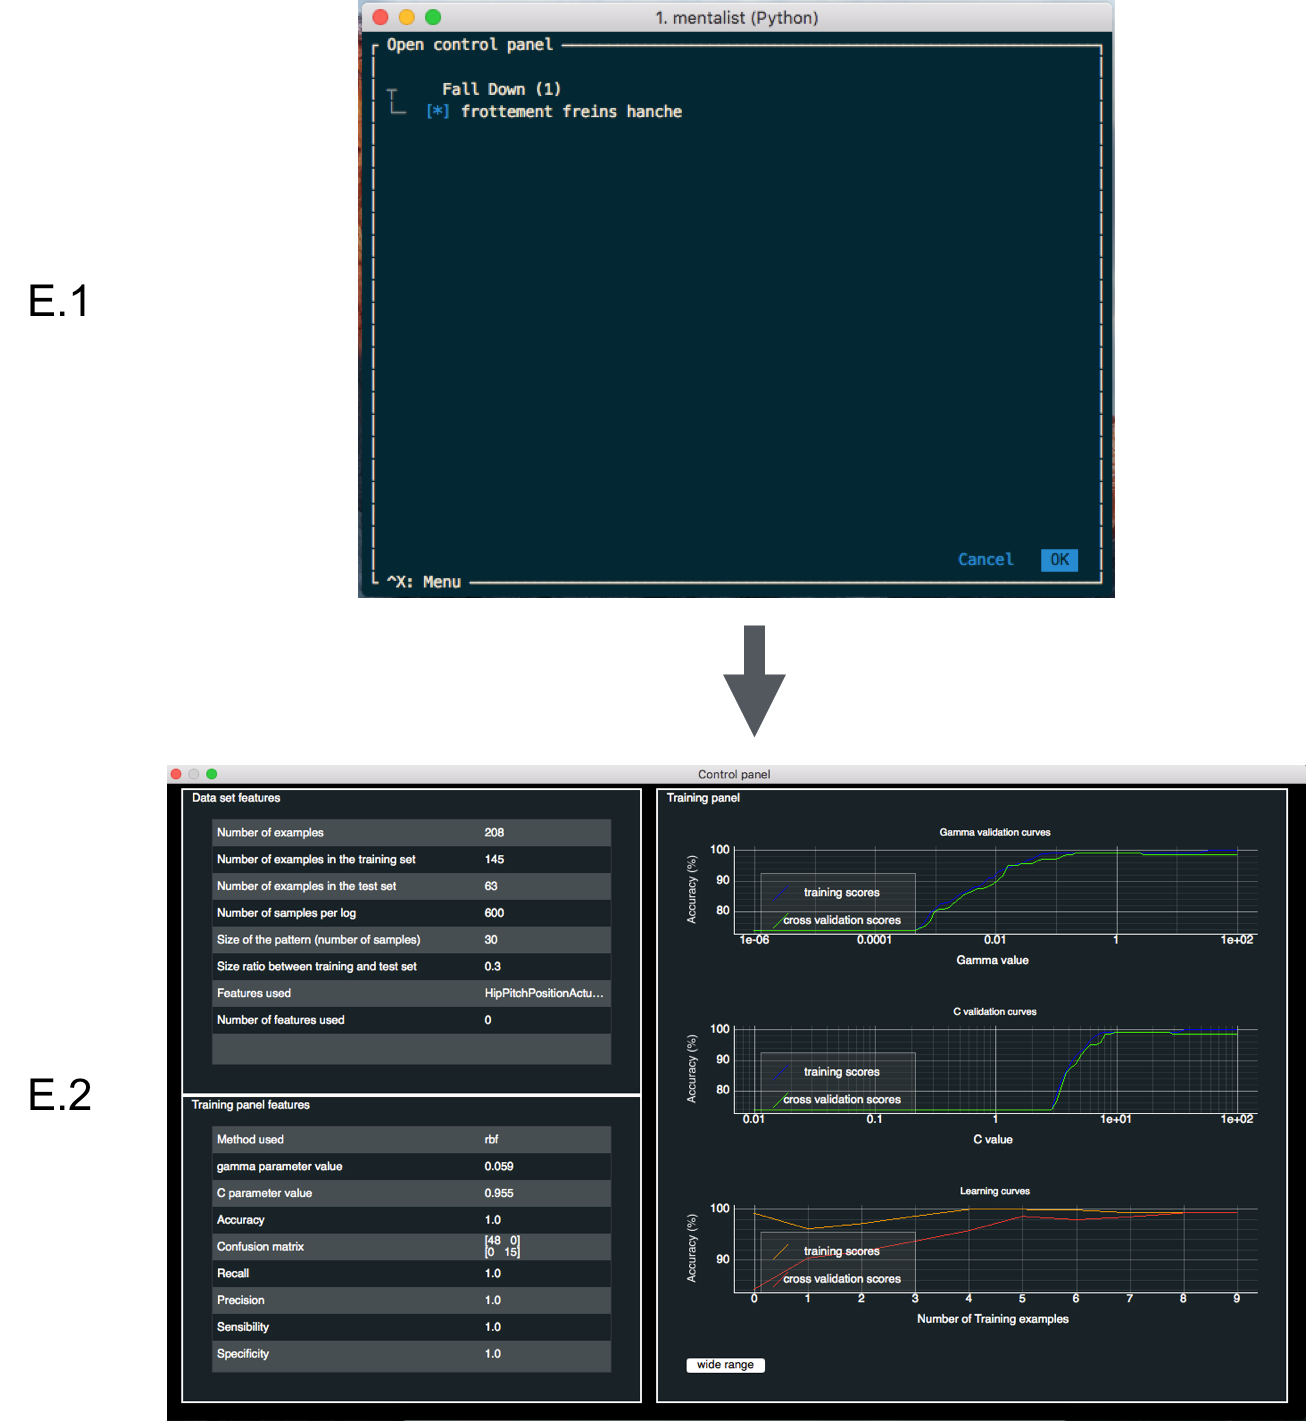
\includegraphics[width=10cm]{images/perf_menu.png}
	\caption[Analyse des performances d'une couche root cause]{Analyse des performances d'une couche root cause.}
	\label{fig: Analyse des performances d'une couche root cause}
\end{figure} 


\subsection{Mise à jour d'une root cause}
\label{Industrialisation du produit: Utilisation suggérée des outils: Mise à jour d'une root cause}
Le menu "Update a root cause"  (cf. figure \ref{fig:Menu principal}) permet d'ajouter des exemples à la base de données d'exemples et d'entrainer de nouveau l'algorithme d'apprentissage afin d'en améliorer les performances. Pour cela, on suit le processus suivant (cf. figure \ref{fig: Analyse des performances d'une couche root cause}) : 
\begin{enumerate}
	\item On sélectionne dans l'arborescence des \emph{errors name} et des \emph{root cause}, la \emph{root cause} que l'on souhaite mettre à jour.
	\item On sélectionne les motifs caractéristiques de la \emph{root cause} dans les exemples ajoutés.
\end{enumerate}

\begin{figure}[H]
	\centering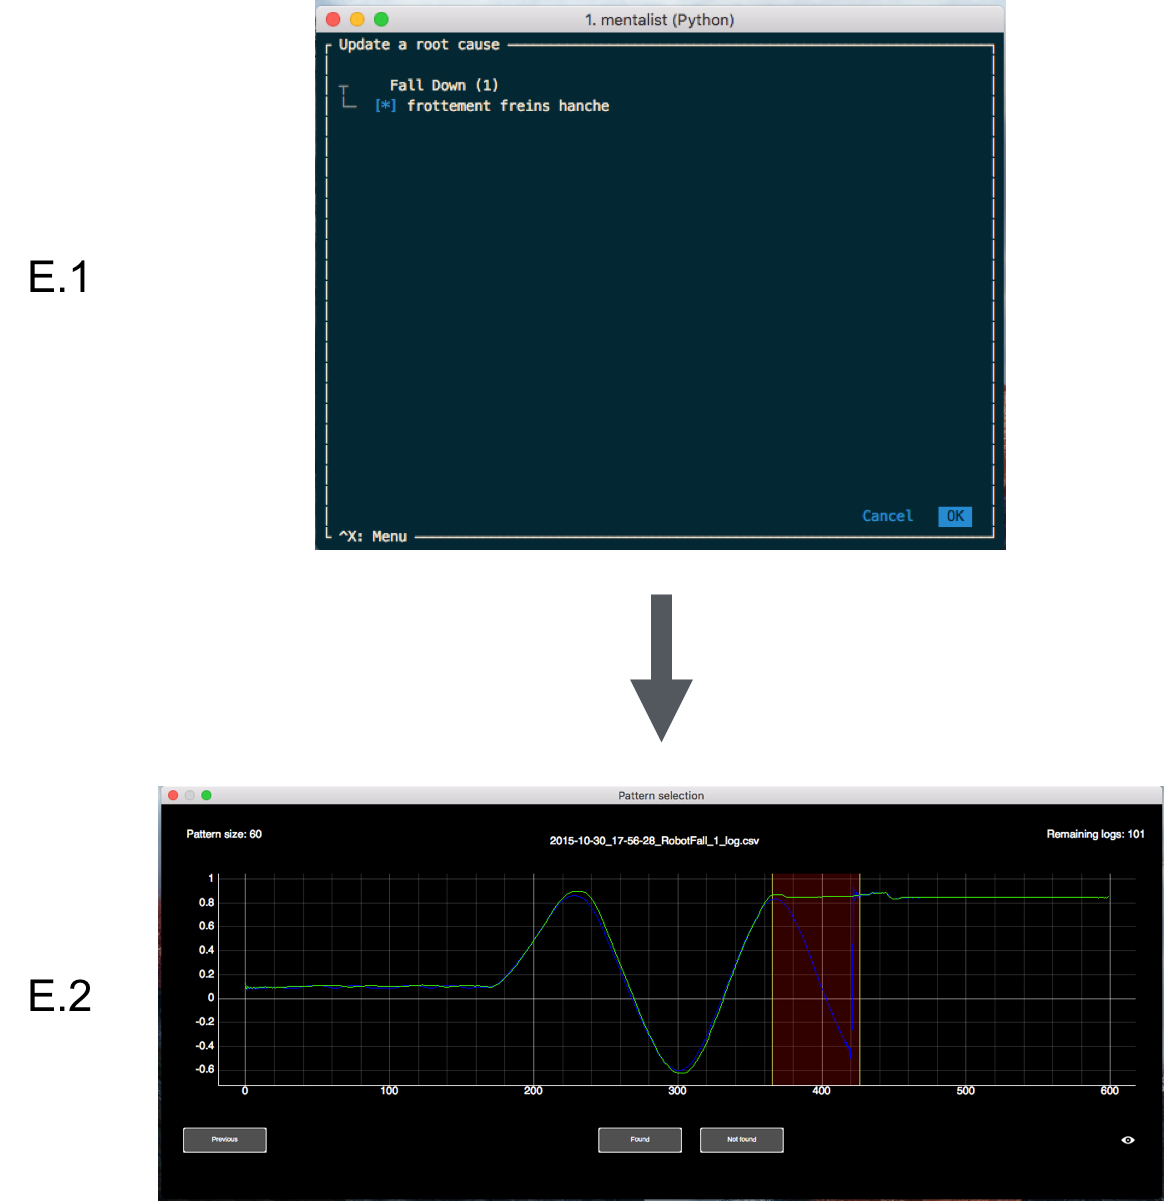
\includegraphics[width=10cm]{images/update_menu.png}
	\caption[Mise à jour d'une root cause]{Mise à jour d'une root cause.}
	\label{fig: Mise à jour d'une root cause}
\end{figure} 


\section{Dimensionnement de la solution}
\label{Industrialisation du produit: Dimensionnement de la solution}
Contrairement à l'étude réalisée en partie \ref{Automatisation du processus d'investigation: Performances de la solution}, on ne désire pas mesurer les performances intrinsèques, mais plutôt l'influence du facteur humain sur celle-ci. On s'intéresse notamment à l'impact qu'a l'évolution de la taille de la région de sélection du Pattern selector (cf. partie \ref{Industrialisation du produit: Outils graphiques: Pattern selection}). En effet, cette variable dépend de la forme du motif, mais également de l'appréciation de l'utilisateur (quand commence le motif, quand se termine-t-il ?). \\
Afin de quantifier cette influence, on effectue plusieurs fois la création de la couche \emph{root cause}  "frottement des freins de la hanche" en augmentant à chaque fois la taille de la région de sélection. On observe la variation de la précision à chaque itération sur le graphique figure \ref{fig: Evolution de la précision de l'algorithme en fonction de la taille de la région de sélection}

\begin{figure}[h]
	\centering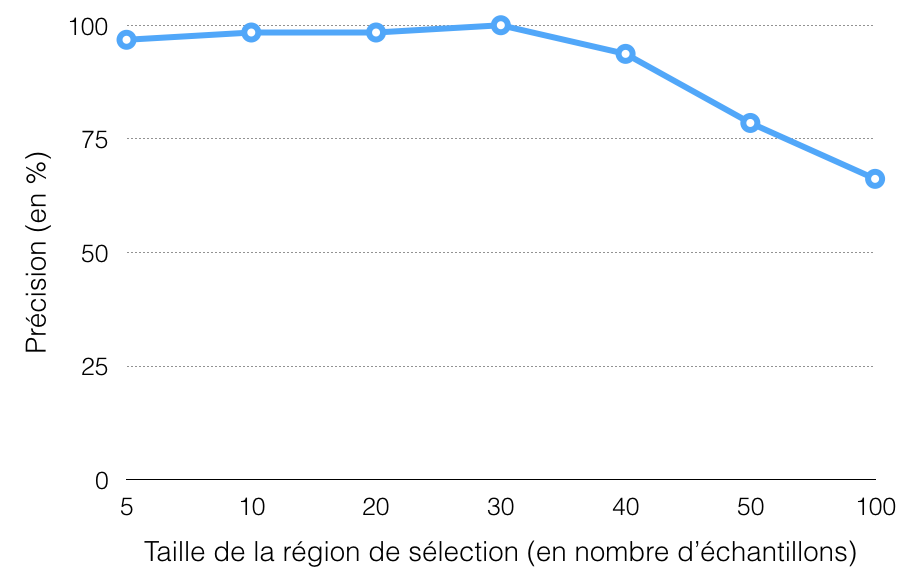
\includegraphics[height=8cm]{images/precision_taille.png}
	\caption[Evolution de la précision de l'algorithme en fonction de la taille de la région de sélection]{Évolution de la précision de l'algorithme en fonction de la taille de la région de sélection.  On observe qu'entre une taille de 10 et 30 échantillons, la précision de l'algorithme augmente légèrement. A partir de 30 échantillons, la précision de l'algorithme diminue.}
	\label{fig: Evolution de la précision de l'algorithme en fonction de la taille de la région de sélection}
\end{figure} 

Au regard des valeurs obtenues, on en déduit que l'algorithme est plus performant lorsque la région de sélection est petite. Or, le but est également de sélectionner le plus précisément possible le motif caractéristique d'une \emph{root cause}. Il faut donc analyser chaque situation au cas par cas,  en gardant en tête ces deux contraintes. Par exemple, si on souhaite apprendre à notre algorithme à reconnaitre une région ayant une taille de 50 échantillons, il sera peut-être plus judicieux d'apprendre l'algorithme à reconnaitre seulement une partie du motif (de 30 échantillons environ).